%%%%%%%%%%%%%%%%%%%%%%%%%%%%%%%%%%%%%%%%%%%%%%%%%%%%%%%%%%%%%%%%%%%%%%%%%%%
% CHEP 2026 proceedings -- CernVM-FS Filebundles
% EPJ Web of Conferences (Web of Conferences LaTeX template)
%%%%%%%%%%%%%%%%%%%%%%%%%%%%%%%%%%%%%%%%%%%%%%%%%%%%%%%%%%%%%%%%%%%%%%%%%%%

\documentclass{webofc}
\usepackage[varg]{txfonts}   % Web of Conferences font
\usepackage{hyperref}
\usepackage{url}
\usepackage{listings}
\hypersetup{colorlinks=true,citecolor=blue,urlcolor=blue,linkcolor=blue}

\newcommand{\cvmfs}{CernVM-FS}
\newcommand{\fuse}{FUSE}
\newcommand{\wlcg}{WLCG}
\newcommand{\filebundle}{\emph{filebundle}}
\newcommand{\Filebundle}{\emph{Filebundle}}
\newcommand{\filebundles}{\emph{filebundles}}
\newcommand{\Filebundles}{\emph{Filebundles}}
% Compact listing style for the JSON bundle example
\lstdefinestyle{bundle}{
  basicstyle=\ttfamily\footnotesize,
  breaklines=true,
  columns=fullflexible,
  frame=single,
  framesep=4pt,
  xleftmargin=4pt,
  showstringspaces=false,
}

\begin{document}

\title{CernVM-FS \Filebundles\ for low-latency software distribution
in interactive use cases}

\author{%
  \firstname{Valentin} \lastname{Volkl}\inst{1}\fnsep\thanks{\email{valentin.volkl@cern.ch}} \and
  \firstname{Georgios} \lastname{Christodoulis}\inst{1} \and
  \firstname{Jakob} \lastname{Blomer}\inst{1}
}

\institute{CERN, 1211 Geneva 23, Switzerland}

\abstract{%
\cvmfs\ is a read-only, on-demand file system used to distribute
scientific software to the Worldwide LHC Computing Grid and many
communities beyond high-energy physics. Its lazy, per-file fetching is
highly efficient for batch computing, but it adds noticeable latency to
interactive sessions: starting an application that requires access to hundreds of
small files on a cold cache is triggering a chain of serial downloading operations to the network.
We present \filebundle\ prefetching, a mechanism that exploits the
predictable file-access pattern at application startup. A small bundle
specification called \filebundle, published next to a trigger file, declares the set of
files needed immediately after the trigger is opened. When a client
opens the trigger, \cvmfs\ prefetches the listed dependencies
concurrently using a pool of worker threads, replacing a long serial
chain of requests with a short parallel prefetch phase. On a ROOT
startup benchmark, \filebundles\ bring performance into the local-disk
range and keep startup time nearly flat as network latency grows, while
the on-demand baseline degrades approximately linearly. \Filebundles\ are
an opt-in feature in \cvmfs\ 2.14.
}

\maketitle

%======================================================================
\section{Introduction}
\label{sec-intro}

\cvmfs~\cite{ref-cvmfs} is a global, read-only file system for
distributing scientific software. 
It is a core component of the Worldwide LHC Computing Grid ( \wlcg\ ) and
is also used by communities beyond high-energy physics, including
Euclid, LIGO, LSST, SKA, and EESSI.

\cvmfs\ uses a distributed architecture (Fig.~\ref{fig-hierarchy}), where software is originally published in a Stratum0 servere - is considered the source of truth, in the form of repositories.
The contents of Stratum0 are then cloned in a series of geographically scattered mirror servers (Stratum1's), arranged to facilitate the different user sites, in order to mitigate the traffic of Stratum0.
Users can access the contents of a repository either directly from a Stratum (0 or 1) (not encouraged) or via a series of forward proxies that site administrators configure, for better load balancing and caching.
\wlcg\ has about fifteen Stratum~1 mirror servers in Europe, the Americas, Australia, and Asia, managing about $3.3\times10^{10}$ files
and 2~PB of data and more than 8000 container images.

Data (repository contents) on \cvmfs\ are stored in a content addressable format.
During publication files are chunked, hashed and compressed.
A filename is associated to its hash (or hashes in the case of chunking) through dedicated metadata dictionaries called catalogs.
Catalogs can also be nested in order to keep catalog operations manageable for large repositories.

From the users perspective, repositories can be accessed via a global namespace, by default under  \emph{/cvmfs} in their machine.
This is done by the \cvmfs\ client, which is a \fuse\ based filesystem.
Typically, there is some disk allocated space in the user's machine that works as a local cache.
\cvmfs\ is performing cache cleanup using an LRU policy; once the quota limit is reached, the cache manager will elect some files for eviction prioritizing those least recently used.
The quota limit is a soft limit, and cleanup efforts will continue until the cache size reaches a specific target (by default half the size of the quota limit). 

For simple listing operations, the client will fetch the associated catalogs which contain all the information necessary.
When an \emph{open()}  is issued from the user, the client will lookup for the correct hash, and will issue a \emph{fetch()}.
During fetching, the client will download the compressed hash, will decompress it and store it in the local cache, available for reading.
On a \emph{read()} the client will make the contents of the files available to the user immediately, or will trigger more \emph{fetch()} operations in case the file is chunked, or the hash has already been evicted from the cache.
According to this mechanism, on first access the cache is empty (cold cache) and the contents of the repository become available after they are needed.
Downloading, decompression, and caching are transparent to the user.


This lazy, content-addressed model is extremely effective for
distributed batch computing, where the benefits of a shared software
distribution system dominate any per-file overhead. In interactive
sessions, however, the same on-demand behaviour can make application
startup noticeably slower than from local disk. This paper presents
\emph{\filebundles}, a mechanism that reduces that startup latency by
prefetching the files an application needs immediately after launch.

\begin{figure}[t]
\centering
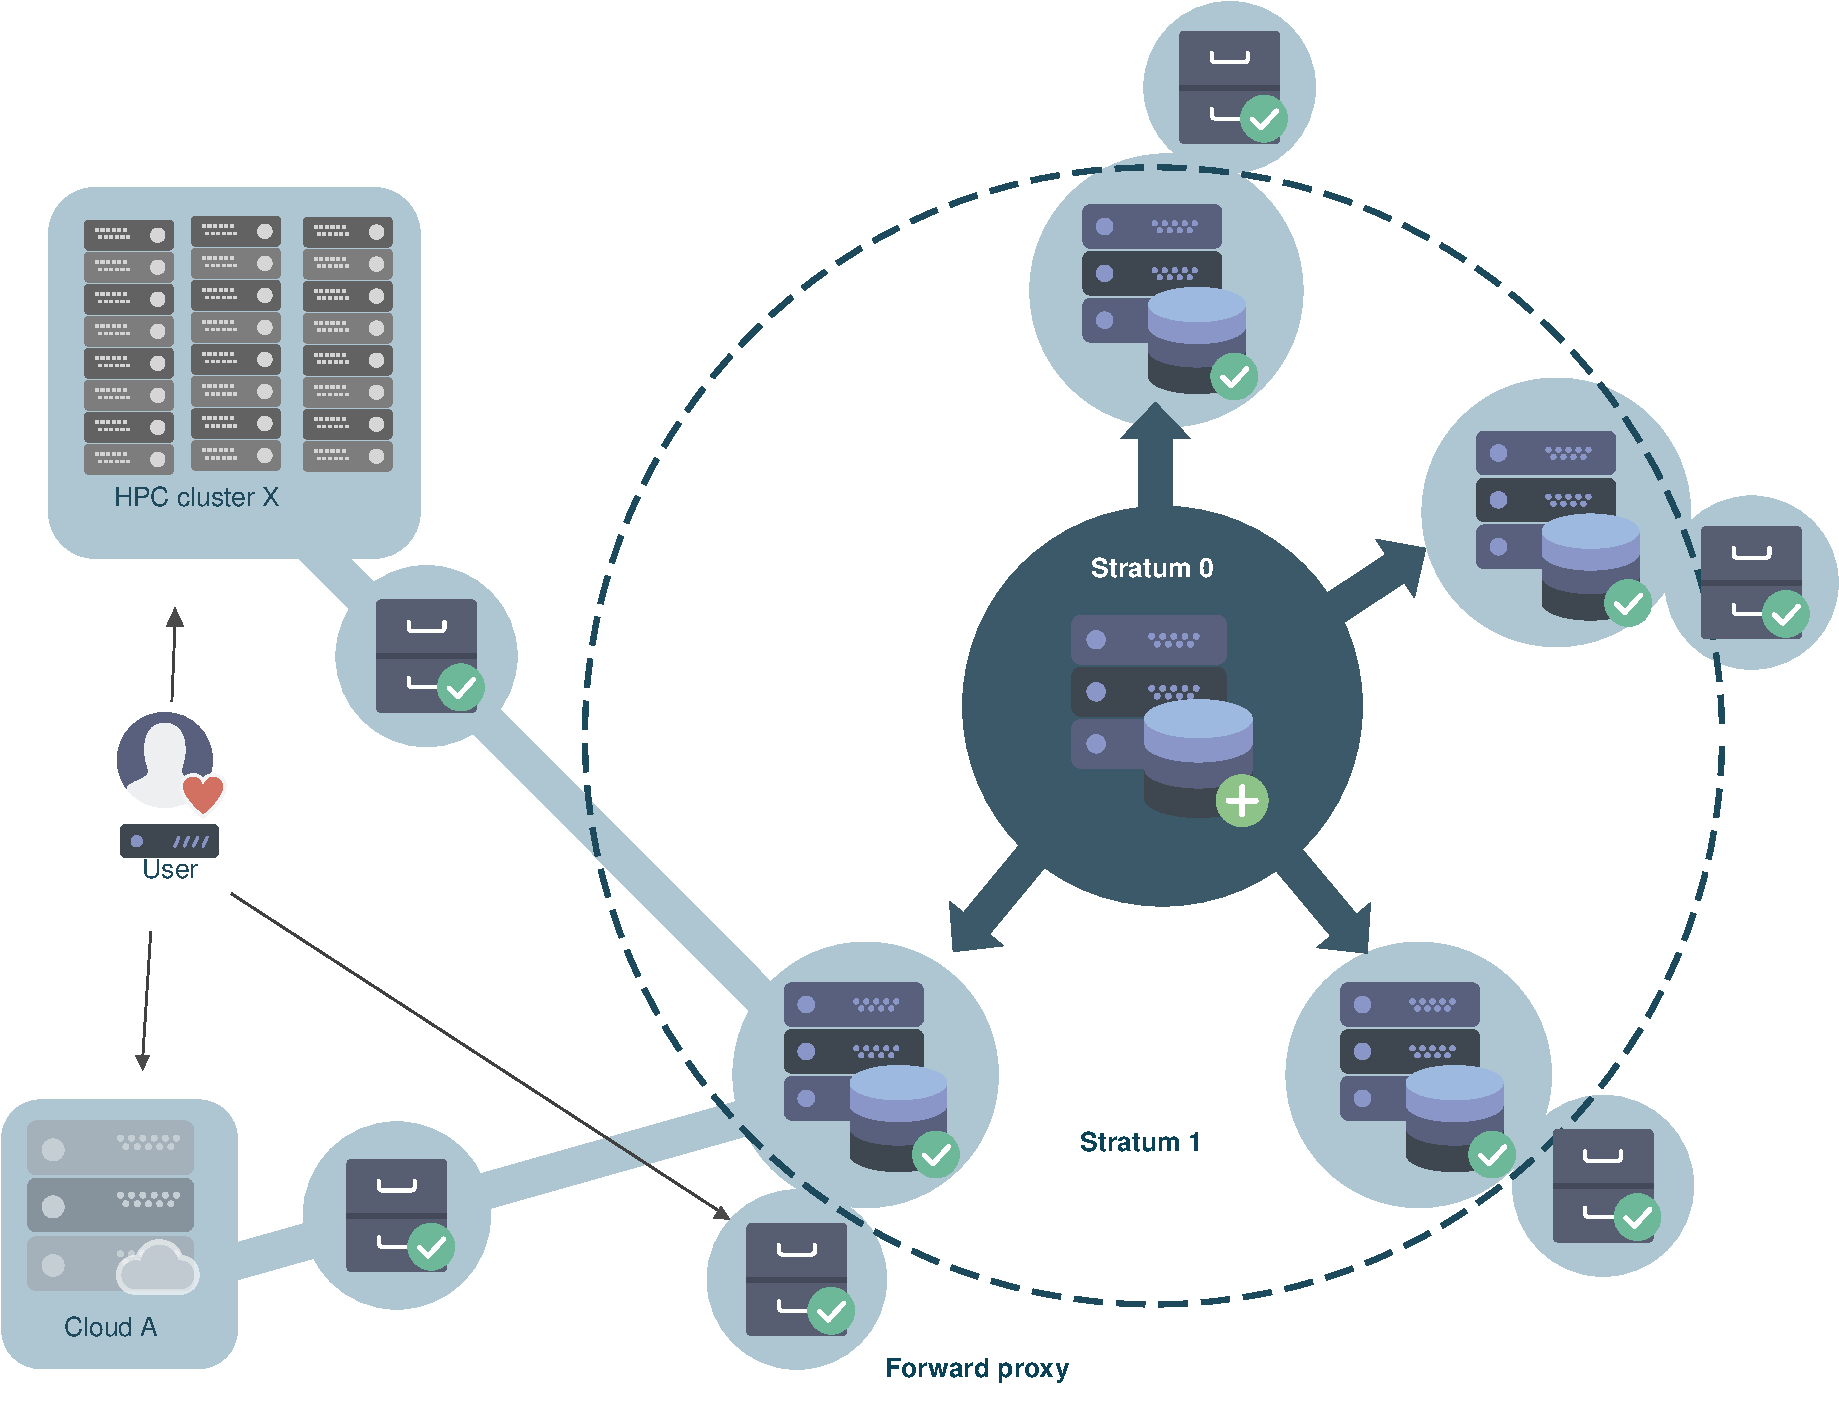
\includegraphics[width=0.78\textwidth]{figures/cvmfs_hierarchy_vectorized.pdf}
\caption{The \cvmfs\ cache hierarchy: a writable Stratum~0 origin,
globally distributed Stratum~1 mirrors, site-level Squid proxies, and
  per-client disk and kernel page caches. The \filebundle\ mechanism operate on the same hierarchy, only changing proxy's workload, creating short bursts of download requests on the first access of a trigger file.}
\label{fig-hierarchy}
\end{figure}
\clearpage % Keep the Section 2 hierarchy figure out of the bundle listing.

%======================================================================
\section{Motivation}
\label{sec-motivation}

\cvmfs\ was designed from the beginning with great emphasis on performance.
Its architecture portends some weak points that have thoroughly been investigated so far.
The first and major one is the overhead added by the network. 
This series of mirror and proxy servers are aiming to improve data locality, opting to minimize its non negligible impact.
The second factor is the overhead added by \fuse\, which is a performance penalty that can not be avoided.
\fuse\ allows the filesystem to be designed in user space, which is a strong requirement by the community (since a kernel module approach is not considered a viable option).

At the CernVM Users Workshop in 2022, Chris Burr (LHCb) reported that
interactive \cvmfs\ use can be roughly three to five times slower
than local disk~\cite{ref-burr}. This overhead is
usually acceptable for distributed batch workloads, but is noticeable
when starting an interactive analysis environment.

The behavior is easy to reproduce on a controlled testbed. Installing
ROOT from a release tarball on local disk, importing ROOT in Python
takes about 2.47~s. Using the same software stack from \emph{/cvmfs}
with a cold cache, the time increases to about 4.69~s. In this setup
the network path is very short, so the slowdown is not primarily a
bandwidth problem. It confirms that a significant part of the delay
comes from the way \cvmfs\ serves many files on demand.

\subsection{Cold cache performance analysis}
\label{sec-time}

When an application such as ROOT starts, it opens many dependent files one after
another. On a cold cache, for each file \cvmfs\ handles a FUSE
upcall, issues an HTTP request, waits for the round trip, downloads the
object, decompresses it , stores it in cache and returns the data. 
This per-file overhead is paid for every dependent file, and is
effectively serialized among the dependencies. 
The per-file amount of work is unremarkable, but the latency across the multiple serialized requests adds up, and becomes noticeable in interactive use.

The idea behind \emph{ \filebundles\ } is that we can take advantage of the fact that the dependencies of an application are or can be known at the time of the publication of the repository, and all dependencies can be fetched simultaneously after the main (trigger) file is opened.
The \filebundle\ mechanism operates within the existing hierarchy of \cvmfs\ (Fig.~\ref{fig-hierarchy}).
There are a couple additional points of complexity that come with the feature conceptually.
From the software maintainers standpoint, there is the responsibility to provide an up to date dependency list during publishing new versions of their software.
For the site infrastructure administrators, there is some change in the proxy access patterns to be anticipated (since on a cold cache, massive parallel download requests will be triggered from the client).

%======================================================================
\section{Filebundles}
\label{sec-design}

\Filebundles\ use prior knowledge of the application's source file dependencies during startup. For applications
such as ROOT~\cite{ref-root} or Python, there is a main file (\emph{ trigger }) whose access is signaling the application's startup.
The series of files that are accessed immediately after the trigger file is opened are often predictable.
A bundle records these dependencies allowing the client to fetch them eagerly in parallel before they are needed from the application.

A bundle is declared by a specification file published next to its
trigger file in the same directory, named
\emph{.cvmfsbundle-<filename>}, where \emph{<filename>} is the
trigger. The specification is a small, versioned JSON document holding
minimal metadata and a flat list of dependency paths, expressed as
absolute paths from the repository root. A representative ROOT bundle,
keyed on the Python package \emph{\_\_init\_\_.py}, contains roughly
250 paths:

\begin{lstlisting}[style=bundle]
#%CVMFS_BUNDLE version=1 encoding=UTF-8
{
  "name": "CVMFS_BUNDLE",
  "version": "1.0.0",
  "encoding": "UTF-8",
  "dependencies": [
    "/root/lib/libCore.so",
    "/root/lib/libRIO.so",
    "/root/lib/libcppyy.so",
    "/root/lib/ROOT/_application.py",
    ...  (~250 paths total)
  ]
}
\end{lstlisting}

When a client receives an \emph{open()} on the trigger file, \cvmfs\ detects the matching
\emph{.cvmfsbundle} specification and begins prefetching the listed
dependencies concurrently, using a pool of worker threads, while the
application continues to run. 
Once fetched, the files (which from the clients point of view is a series of compressed hashes) are getting decompressed (also in parallel) and stored in the local disk.
In effect, a long serial chain of
dependent requests is replaced by a much shorter parallel prefetch
phase that warms the local cache ahead of the application's subsequent
\emph{open()} calls.

The feature is disabled by default and can be enabled per mountpoint with the configuration parameter
\emph{CVMFS\_PREFETCH\_FILEBUNDLES=yes}~\cite{ref-docs}. The setting
is read at mount time; mounts for which it is disabled do not start
bundle prefetching. The prefetch-pool size is controlled by
\emph{CVMFS\_BUNDLE\_POOL\_SIZE}.

\subsection{Publishing a filebundle}
\label{sec-publish}

In order to create \emph{.cvmfsbundle-<filename>}, there is a straightforward series of steps.
First, choose a suitable trigger file, for example a Python
\emph{\_\_init\_\_.py} or a launcher binary such as
\emph{root.exe}. Second, determine which files are typically read
after that trigger; this can be done by hand or with tracing tools such
as \emph{strace} or the built-in \emph{CVMFS\_TRACEFILE}
mechanism. Third, publish the resulting \emph{.cvmfsbundle-<filename>}
specification next to the trigger file, just like any other file in the
repository. Removing the specification (and republishing) removes the
bundle, after which the trigger behaves like an ordinary file.

%======================================================================
\section{Results}
\label{sec-results}

Unless noted otherwise, the benchmarks use ROOT~6.36.12 in a test
\cvmfs\ repository served from \emph{localhost}. The client ran on
an AMD EPYC~7302 system (2$\times$16 cores, 64 threads at
${\sim}3.0$~GHz, 251~GB RAM), with AlmaLinux~10.1 and kernel~6.12.
Using \emph{localhost} removes external network effects, exposing the
per-file software overhead.

\subsection{Startup performance}
\label{sec-startup}

Figure~\ref{fig-violin} compares ROOT startup times on local disk, on 
\cvmfs\ with a cold cache and no \filebundles, and on \cvmfs\ with
\filebundles\ enabled. In this benchmark, \filebundles\ bring \cvmfs\
startup time to the local-disk range. Some measurements are marginally
faster than local disk, consistent with overlap between downloading and
decompression in the prefetch path.

\begin{figure}[t]
\centering
\includegraphics[width=0.62\textwidth]{figures/violin_bundle.pdf}
  \caption{A violin plot of the distribution of startup times over ten repetitions of importing ROOT. With \filebundles\ enabled
(\emph{CVMFS\_PREFETCH\_FILEBUNDLES=ON}), \cvmfs\ startup matches
local-disk performance, closing the gap to the on-demand cold-cache
baseline.}
\label{fig-violin}
\end{figure}

\subsection{Prefetch thread pool}
\label{sec-pool}

An efficient prefetching mechanism should ensure that the files inside the bundle are fetched as rapidly as possible to be available on potential access.
During our primitive experiments, we realized that a single-threaded fetching mechanism inside the client is getting saturated and the network is being underutilized ( every download is followed by a decompression from the same worker thread ).
To overcome this bottleneck, we implemented prefetching with a pool of worker threads whose size is
set by \emph{CVMFS\_BUNDLE\_POOL\_SIZE}. As shown in
Fig.~\ref{fig-pool}, startup performance improves as workers are added
and saturates around eight threads, which is also the default. Most of
the benefit is therefore obtained with a moderate amount of concurrency
and without aggressive tuning.

\begin{figure}[t]
\centering
\includegraphics[width=0.62\textwidth]{figures/pool_scan.pdf}
\caption{ROOT startup time as a function of the prefetch thread-pool
size (\emph{CVMFS\_BUNDLE\_POOL\_SIZE}). Performance saturates around
eight worker threads, the default.}
\label{fig-pool}
\end{figure}

\subsection{Network latency}
\label{sec-latency}

For the experiments of section ~\ref{sec-pool} shown in Fig.~\ref{fig-pool}, the repository was served from localhost, which minimizes the effect of network latencies that appear on more realistic scenarios.
To comprehend the impact of network latency to the performance of \filebundles, we injected loopback round-trip latency with \emph{tc qdisc netem}.
Without \filebundles, startup time grows approximately linearly with
round-trip time because the latency of the sequential dependent small-file fetches grows cumulatively.
With \filebundles, startup time remains nearly flat
over a substantial range (Fig.~\ref{fig-latency}): concurrent prefetch
pays the round-trip penalty for a small number of batches rather than
for each file. This is an idealized loopback experiment.

\begin{figure}[t]
\centering
\includegraphics[width=0.62\textwidth]{figures/latency_scan.pdf}
\caption{ROOT startup time as a function of injected round-trip
latency. The on-demand baseline degrades roughly linearly, while
\filebundles\ keep startup nearly flat by overlapping requests.}
\label{fig-latency}
\end{figure}

\subsection{Caveats}
\label{sec-caveats}

\Filebundles\ do not reduce the total amount of data transferred; they
compress the startup traffic into a short, intense burst. In the
benchmark, requests peak at about 1480~per~second with \filebundles,
versus about 680~per~second without them (Fig.~\ref{fig-burst}). The
feature should therefore be used selectively, targeting
interactive systems such as \emph{lxplus}, where startup latency
matters most. Over-prefetching should be avoided, and any rollout
should be coordinated with proxy and site administrators so that the
request bursts do not overload the sites' proxies.

\begin{figure}[t]
\centering
\includegraphics[width=0.62\textwidth]{figures/req_burst.pdf}
\caption{Request rate during startup. \Filebundles\ concentrate the same
total traffic into a shorter, more intense burst (peak ${\sim}1480$
req/s versus ${\sim}680$ req/s without bundles).}
\label{fig-burst}
\end{figure}

%======================================================================
\section{Outlook}
\label{sec-outlook}

\cvmfs\ since version 2.14 takes advantage of the \fuse\ passthrough mechanism introduced in the linux kernel version 6.9 (available in EL10 and on), and can hand over to the
kernel a descriptor for the cached backing file during \emph{open()}, so
subsequent reads bypass FUSE. 
This feature works only for unchunked files and eliminates the overhead imposed by the \fuse\ call hierarchy. 
Its potential to improve the startup time of application combined with \filebundles\ still
needs to be benchmarked. Planned work for \cvmfs~2.15 includes tools
for creating and updating bundles, support for file chunks in bundle
specifications, and integration with build tools. Packfiles, which
would combine small backend objects to reduce request counts, are also
under consideration; backward compatibility is the principal obstacle.

%======================================================================
\section{Conclusions}
\label{sec-conclusions}

\Filebundles\ reduce application-startup latency when a known set of files
is needed immediately after a trigger is opened. They require the
repository maintainer to trace startup behaviour and publish a
\emph{.cvmfsbundle} specification next to the trigger. In the ROOT
benchmark, they reduce cold-start time to the local-disk range and make
startup less sensitive to added round-trip latency. \Filebundles\ are an
opt-in \cvmfs~2.14 feature, enabled per mount with
\emph{CVMFS\_PREFETCH\_FILEBUNDLES}. They are best suited to
interactive systems, where the prefetch burst can be managed.

\vspace{0.5em}
\noindent\textbf{Acknowledgements.} We thank Chris Burr (LHCb) for the
valuable input that provided a measurable reference for the potential of improving applications' startup on interactive workloads.

\vspace{0.3em}
\noindent\emph{Disclosure: AI-based tools were used to assist with
drafting and formatting this manuscript; all content was reviewed and
verified by the authors.}

%======================================================================
\begin{thebibliography}{9}

\bibitem{ref-cvmfs}
J. Blomer, C. Aguado-S\'anchez, P. Buncic, A. Harutyunyan,
Distributing LHC application software and conditions databases using
the CernVM file system, J.\ Phys.: Conf.\ Ser.\ \textbf{331}, 042003
(2011). \url{https://doi.org/10.1088/1742-6596/331/4/042003}

\bibitem{ref-burr}
C. Burr, \textit{Client performance}, CernVM Users Workshop (2022).
\url{https://indico.cern.ch/event/1079490/contributions/4939521/attachments/2506388/4306645/2022-09-12_CVMFS-Workshop_LHCb.pdf}

\bibitem{ref-root}
R. Brun, F. Rademakers, ROOT---an object oriented data analysis
framework, Nucl.\ Instrum.\ Methods Phys.\ Res.\ A \textbf{389},
81--86 (1997). \url{https://doi.org/10.1016/S0168-9002(97)00048-X}

\bibitem{ref-docs}
\cvmfs\ documentation. \url{https://cvmfs.readthedocs.io/}

\end{thebibliography}

\end{document}
